\chapter{心电信号及其特征参数 }
\section{心电信号的产生机理与特点}
\subsection{心电信号的产生机理} 
心脏是人体血液循环系统中的重要器官,血液能在人体封闭的循环系统中不停的流动依赖于心脏永不停歇的节律性的收缩与扩张,
才能完成相应的气体交换,从而维持了人体生命活动的最基本要求\cite{8}。 
\begin{figure}[htbp]
    \centering
    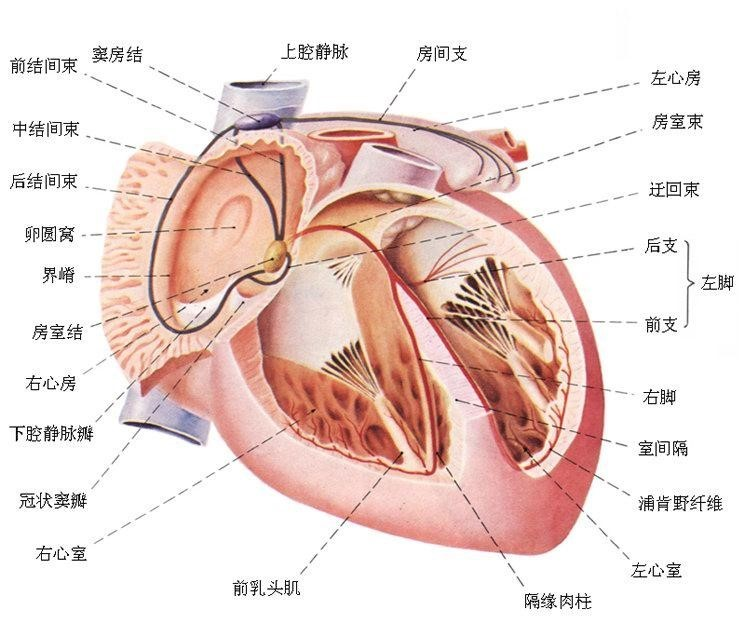
\includegraphics[width=.6\linewidth]{301}
    \caption{\label{fig:301}心脏的传导模式}
\end{figure}

人体心脏的传导模式如\autoref{fig:301}所示。在正常人体内,由窦房结发出的一次兴奋,按一定的途径和时序,依次传向心房和心室,引起整个心脏的兴奋。
位于上腔静脉和右心房的交界处的窦房结是人体心脏的原发性起博兴奋点。正常情况下,由窦房结的起博细胞每分钟自发地产生 50~100 次可传导的动作电位。
该动作电位以有序方式通过心房内的传导束,先后激活右心房与左心房。兴奋通过房室结经短暂延时后进入希氏束,左、右束支到达大而特化的传导细胞系统——普金野氏网。
最后兴奋通过普金野氏网迅速激动心室壁的普通工作性心肌细胞。一次正常的心博动过程就是伴着电兴奋波传播到整个心脏从而完成的。 

因此,每一个心动周期中,心脏各部分兴奋过程中出现的电变化的方向、途径、次序和时间等,都有一定的规律。这种由大量心脏细胞有序活动产生的生物电变化
通过心脏周围的导电组织和体液,传导到身体表面上来,使人体各部位在每一心动周期中也都发生有规律的变化。
目前临床上记录的心电图就是在人体表面的一定部位放置测量电极记录下来的心脏电变化曲线。心电图集中反映心脏兴奋的产生、传导和恢复过程中的一系列生物电变化。 
\subsection{心电信号的特点}
(1)	幅值低 

心电信号幅值非常低,一般为 mv 数量级,常见范围为 0.05~5mV,典型值为 l mV。 
同其他生物医学信号一样,心电信号的检测,必须依赖与高输入阻抗、高共模抑制比的心电检测放大电路,并做好相应的进行滤波去噪工作。 

(2)	频率低 

与幅值一样,心电信号频率也在较低的频率范围之内,常见频谱范围为 0.05~100Hz,而相应的心电信号能量则主要集中在 0.5~20Hz。 

(3)	易受干扰性 

人体是复杂的生命体,从个体的角度来说,人体内各器官各部位之间存在着相互影响,从整体的角度来说,人体在与外界环境的交互中易受环境的影响。
除此之外,个体间心脏位置、呼吸、年龄、身体状况等差异都会使检测得到的心电信号发生相应的变化。 

\section{心电信号基本特征及其生理意义}
正常的人体心电活动会引起一系列的电位变化,在心电图上表现为相应的波段,如\autoref{fig:302}所示\cite{9}。 
\begin{figure}[htbp]
    \centering
    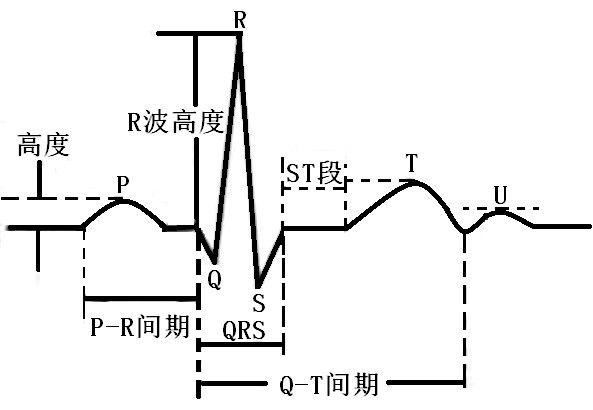
\includegraphics[width=.6\linewidth]{302}
    \caption{\label{fig:302}心电典型波形}
\end{figure}

(1)	P 波:反映了左右心房的电激动过程中电位随时间的变化,通常在心动周期中最先出现。其持续时间为兴奋在左、右心房扩布的时间,持续 0.04~0.11 秒。 

(2)	P-R 间期:代表心房开始除极至心室开始除极的时间,即 P 波与 QRS 波群起点的间隔。其值随年龄和心率而略有差别,正常人一般在 0.12s-0.20s 之间。 

(3)	QRS 波群:反映左右心室除极过程电位和时间的变化,其波形直接反映心室的搏动状况。QRS 波群形态变化比较大,正常心电图中 QRS 波群第一个出现是负向的 Q 波,
随后是高幅度并突尖的 R 波,R 波之后是负向的 S 波。正常 QRS 时间在 0.06s-0.08s 之间,一般不超过 0.10s。 

(4)	ST 段:代表心室除极后缓慢复极的过程。正常情况下 ST 段时间在0.12-0.16s。 

(5)	T 波:与 ST 段相反,T 波反映晚期心室复极过程电位的变化。通常形圆钝,持续时间较长,形态多样。 

(6)	U 波:U 波的形成具体原理目前没有统一结论,可能表示心肌激动后的电位变化,为 T 波后的一个小波,方向与 T 波相同,一般在 V3 导联最为明显。 

(7)	Q-T 间期:反映心室除极和复极的总时间,其值通常为 0.32s-0.44s。 

\section{心电信号常见干扰}

如前所述,人体心电信号是一种弱电生物医学信号,具有低频率、低幅值易受外界各种信号的干扰等特性。一般正常的心电信号频率范围为 0.05-100Hz,而 90\%
的心电信号频谱能量集中在 0.25-35Hz 之间。临床上实际采集心电信号时通常会伴有各类干扰噪声,具体而言,噪声来源可分为以下几类: 

(1)	工频干扰 

市电电压的频率为 50Hz,它会以电磁波的辐射形式,对电气设备和电子设备造成干扰,导致设备运行结果异常。工频干扰的模型由 50Hz 的正弦信号及其谐波组成。
幅值通常与 ECG 峰峰值相当或更强。 

(2)	电极接触噪声 

电极接触噪声是瞬时干扰,来源于电极与人体肌肤的接触不良,电极接触噪声可抽象为快速、随机变化的阶跃信号,它按指数形式衰减到基线值,包含工频成分。其幅值可达记录仪的最大值。 

(3)	人为运动 

人为运动会引起电极与皮肤阻抗改变,导致瞬时的基线改变,基线干扰形状可认为类似周期正弦信号,其峰值幅度和持续时间是变化的,幅值通常为几十毫伏。 

(4)	肌电干扰 

肌电干扰来自于人体的肌肉颤动,可视为瞬时发生的零均值带限噪声,幅值一般不明显,主要能量集中在 30-300Hz 范围内。 

(5)	基线漂移和呼吸 

基线漂移和呼吸时造成的干扰一般由人体呼吸、电极移动等低频干扰所引起,频率小于 50 Hz,可视为一个加在心电信号上的与呼吸频率同频率的正弦分量。 

\section{本文心电数据来源}

本文中主要参考使用了 MIT-BIH 心率不齐数据库,作为目前国际上公认的可作为标准的三大心电数据库之一,MIT-BIT 心律不齐数据库近年来应用比较广泛
该数据库一共记录了 48 组心律不齐数据,每组数据包含两个导联,记录时间长达半个小时,采样率为 360Hz,并且伴有人工注释。 
如\autoref{fig:303}所示,MIT-BIH 数据库每组数据包含***.atr、***.dat、***.hea 三个文件。扩展名为.dat 的文件是数据文件,
扩展名为.atr 的文件为注释文件,扩展名为.hea 的文件为头文件。头文件存储方式为 ASCII 码字符,详细说明了与它关联的数据文件的名字及其属性。数据文件是按二进制存储的,以自定义的格式记录了信号原始数据。注释文件
以二进制存储格式,记录了心电诊断专家对信号分析的结果。 
\begin{figure}[htbp]
    \centering
    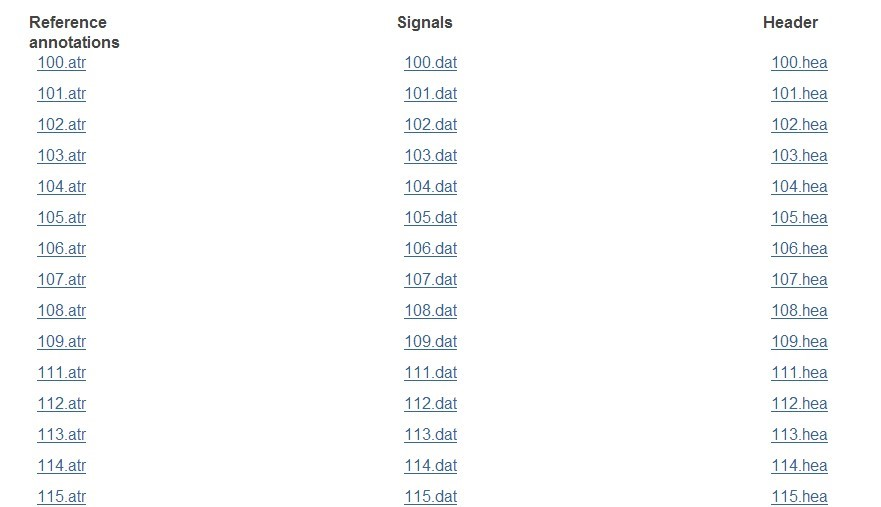
\includegraphics[width=.6\linewidth]{303}
    \caption{\label{fig:303}MIT-BIH心电数据库文件(部分)示意 }
\end{figure}

\section{心电信号数据的准备 }
在进行相关心电分析之前,需要获取相关数据。本节在前人的基础上\cite{10},通过 Matlab 编程对 MIT-BIH 数据库的文件进行了数据提取。
下文以 100.hea 、100.dat、100.atr 为例就基本原理与具体实现步骤说明如下: 

(1)	hea 文件的识读 

如\autoref{fig:304}所示,头文件中包含的信息有记录行、信号规范行及注释行。记录行包括信号名称、片段数(可选)、信号数量、采样频率等信息。
信号技术规范行包括储存信号的文件名、储存格式、ADC 增益、基线值、ADC 分辨率、ADC 零值、信号初始值等
信息。注释行以“\#”开始,简单说明患者的信息。 
\begin{figure}[htbp]
    \centering
    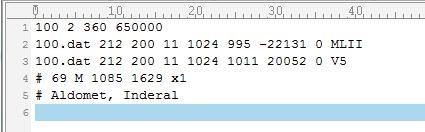
\includegraphics[width=.6\linewidth]{304}
    \caption{\label{fig:304}100.hea 文件示意}
\end{figure}

(2)	dat 文件的识读 

MIT-BIH 数据库中数据存储的格式包括 Format212 等八种。其中 Format212 原理是按照采样顺序,对两通道数据(为方便说明,设定其为信号 0 与信号 1)
进行交替存储,每三个字节存储两个数据,其中信号 0 的数据取自第一字节对的低 12 位,信号 1 的数据由第一字节对的剩余 4 位与下一字节的 8 位共同组成。
\autoref{fig:305}显示了 100.dat 的十六进制显示的数据片段。按照 212 的格式,从第一字节读起的三个字节的数据为“E3 33 F3”,则两通道信号值分别为 0x3E3 与 0x3F3,
对应的十进制值分别为 995 与 1011,乘上 ADC 增益数值所得的最后结果为 4.975mV 与 5.055mV。 
\begin{figure}[htbp]
    \centering
    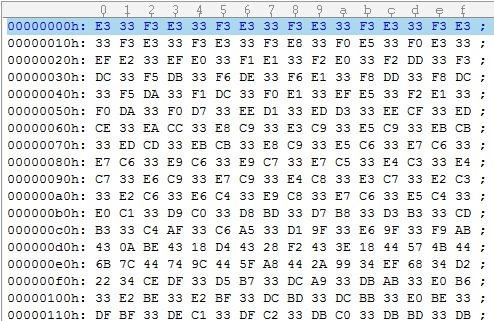
\includegraphics[width=.6\linewidth]{305}
    \caption{\label{fig:305}100.dat 文件(部分)示意 }
\end{figure}

(3)	atr 文件的识读 

atr 文件的识读与 dat 文件类似,由于不涉及原始数据,故在此不做过多介绍。 

按照上述方法,对 MIT-BIH 的原始数据进行处理,本文将处理后获得的数据按照每行保存一个心电样本数据的形式以文本格式(.txt)进行了存储供 Android 分析使用。
\autoref{fig:305}给出了 113.dat 文件提取的 2 通道数据的波形,相应的 txt 文档如\autoref{fig:306}所示。 

\begin{figure}[htbp]
    \centering
    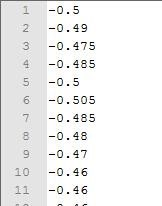
\includegraphics[width=.4\linewidth]{307}
    \caption{\label{fig:306}MIT-BIH 113.dat 的 2 通道心电数据波形(部分)}
\end{figure}

\begin{figure}[htbp]
    \centering
    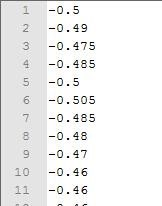
\includegraphics[width=.4\linewidth]{307}
    \caption{\label{fig:307}Android 进行分析处理的输入数据文件示意}
\end{figure}

\section{本章小结}
本章主要对心电进行了概述。首先阐述了心电信号的产生与心电图测试的原理,同时说明了心电信号的低频、微弱、不稳定的特点。其次,对心电波形的心电信号
基本特征及其生理意义进行了说明。再次,对心电信号分析检测过程中易出现的干扰与噪声进行了说明。最后,介绍了本文数据来源 MIT-BIH 数据库,并介绍了对其文件进行数据
提取的原理。 
